\documentclass[letterpaper, 11pt, oneside]{memoir}
\usepackage{fontspec}

%%%%%%%%%%%%%%%%%%%%%%%%%%%%%%%%%%%%%%%%%%%%%%%%%%%%%%%%%%%%%%%%%%%%%%%%%%%%%%%
% BEG: PACKAGES
%
\usepackage{geometry}
\usepackage{graphicx}
\usepackage{tikz}
\usetikzlibrary{calc, fadings, positioning, shadings}
\usepackage{url}
\usepackage{xcolor}
% END: PACKAGES
%%%%%%%%%%%%%%%%%%%%%%%%%%%%%%%%%%%%%%%%%%%%%%%%%%%%%%%%%%%%%%%%%%%%%%%%%%%%%%%

%%%%%%%%%%%%%%%%%%%%%%%%%%%%%%%%%%%%%%%%%%%%%%%%%%%%%%%%%%%%%%%%%%%%%%%%%%%%%%%
% BEG: COLOR/TEXT/FONT CONFIGURATION
%

\setmainfont{SourceSerifPro-Regular}[
  BoldFont = SourceSerifPro-Bold,
  ItalicFont = SourceSerifPro-It,
]
\setsansfont{SourceSansPro-Regular}[
  BoldFont = SourceSansPro-Bold,
  ItalicFont = SourceSansPro-It,
]
\setmonofont{SourceCodePro-Regular}[
  BoldFont = SourceCodePro-Bold,
  ItalicFont = SourceCodePro-It,
]

\definecolor{Orange}{cmyk}{0, 0.40, 0.80, 0}
\definecolor{RichBlack}{cmyk}{0.25, 0.25, 0.25, 0.70}

\tikzfading[name=fade lightly right,%
            left color=transparent!0,%
            middle color=transparent!0,%
            right color=transparent!25]

%
% END: TEXT/FONT CONFIGURATION
%%%%%%%%%%%%%%%%%%%%%%%%%%%%%%%%%%%%%%%%%%%%%%%%%%%%%%%%%%%%%%%%%%%%%%%%%%%%%%%

%%%%%%%%%%%%%%%%%%%%%%%%%%%%%%%%%%%%%%%%%%%%%%%%%%%%%%%%%%%%%%%%%%%%%%%%%%%%%%%
% BEG: DOCUMENT CONFIGURATION
%

\preauthor{\rmfamily\Large\begin{center}}
\postauthor{\end{center}}
\predate{\rmfamily\small\begin{center}} \postdate{\end{center}}

% Chapter Styling
\renewcommand{\chaptername}{Lab}
\chapterstyle{veelo}

%
% END: DOCUMENT CONFIGURATION
%%%%%%%%%%%%%%%%%%%%%%%%%%%%%%%%%%%%%%%%%%%%%%%%%%%%%%%%%%%%%%%%%%%%%%%%%%%%%%%

%%%%%%%%%%%%%%%%%%%%%%%%%%%%%%%%%%%%%%%%%%%%%%%%%%%%%%%%%%%%%%%%%%%%%%%%%%%%%%%
% BEG: DOCUMENT METADATA
%


%
% END: DOCUMENT METADATA
%%%%%%%%%%%%%%%%%%%%%%%%%%%%%%%%%%%%%%%%%%%%%%%%%%%%%%%%%%%%%%%%%%%%%%%%%%%%%%%

\begin{document}

%%%%%%%%%%%%%%%%%%%%%%%%%%%%%%%%%%%%%%%%%%%%%%%%%%%%%%%%%%%%%%%%%%%%%%%%%%%%%%%
% BEG: TITLE PAGE
\newgeometry{margin=0.5in, marginparsep=0in}
\thispagestyle{empty}
\begin{titlingpage}
\begin{tikzpicture}[remember picture, overlay, x=1in, y=1in]
  \node[inner sep=0pt, anchor=north west, scope fading=south] at (current page.north west) {%
    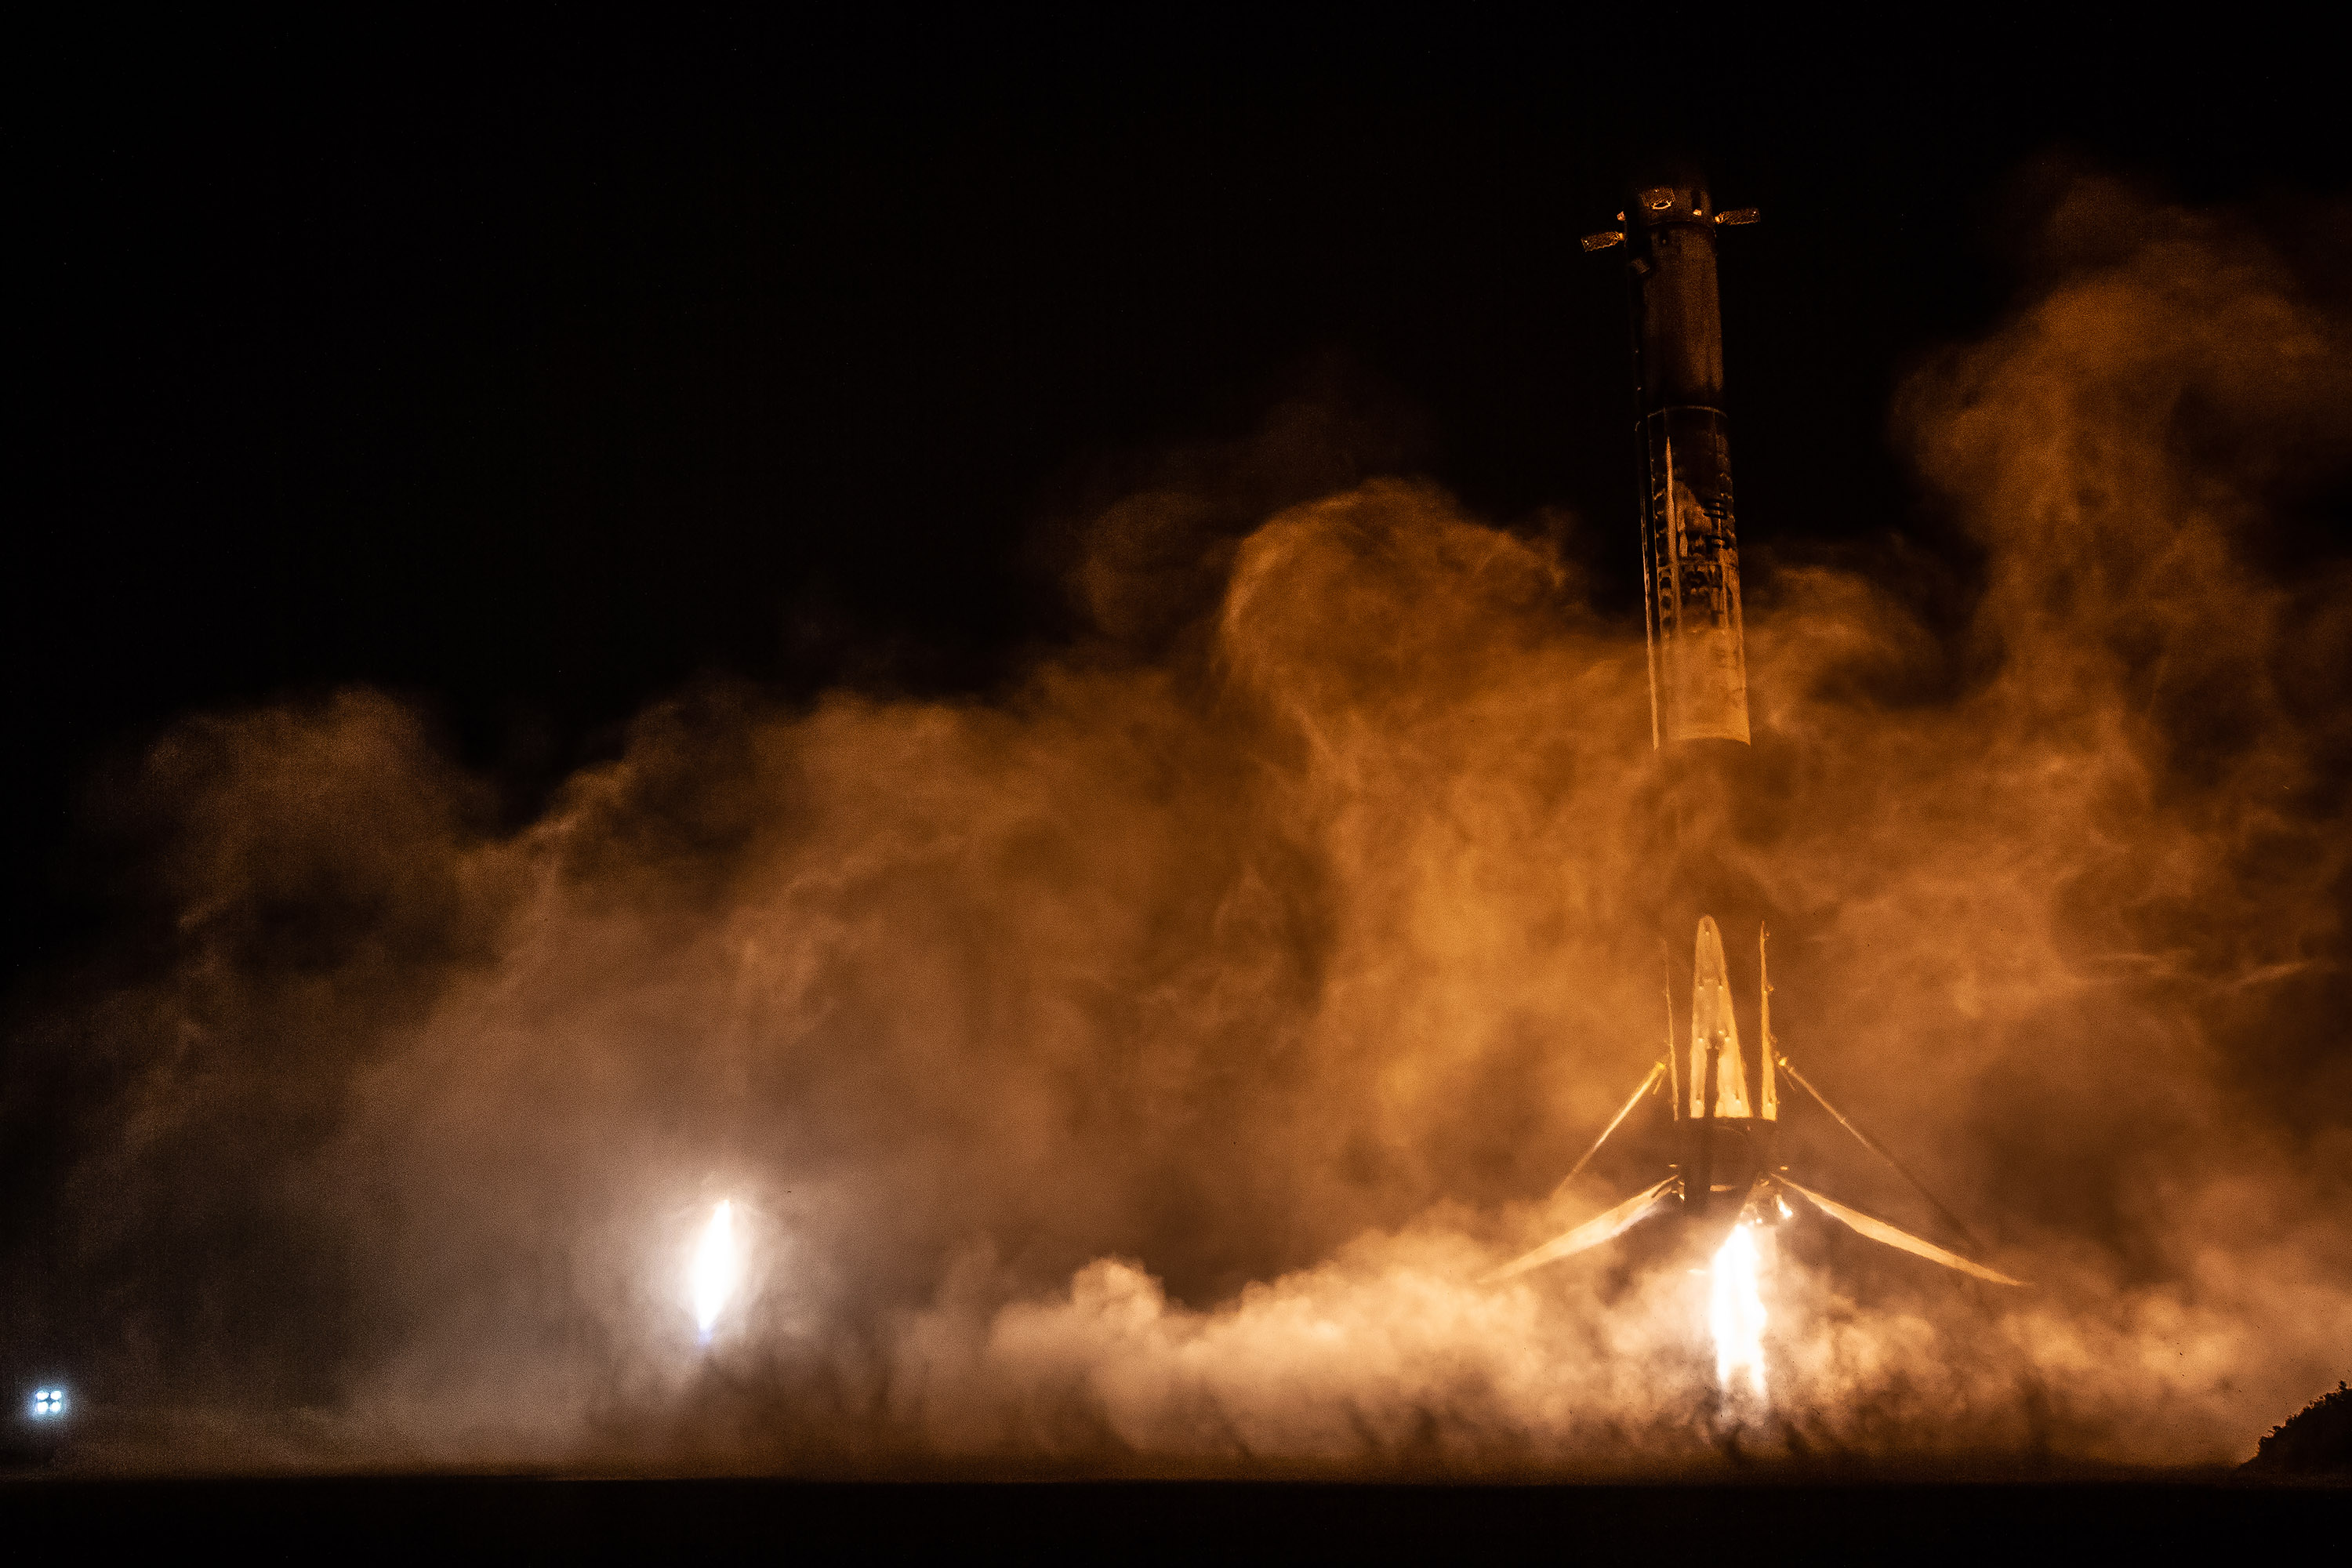
\includegraphics[%
      height = 9.5in,%
      trim = 300 20 0 50,
      clip%
    ]{images/STP-2-Mission-Landing}%
  };

  \node [at={($(current page.north west)+0.5*(1, 0)$)}] (A1) {};
  \node [at={($(current page.south west)+1.0*(1, 0)$)}] (A2) {};
  \node [at={($(current page.south west)+2.0*(0, 1)$)}] (B) {};
  \node [at={($(current page.south east)+0.5*(0, 1)$)}] (C) {};

  \fill [color={Orange}, path fading={fade lightly right}]
    (A1)
    rectangle
    (A2);

  \fill [color={RichBlack}]
    (current page.south west)
    rectangle
    (A1);
  \fill [color={RichBlack}]
    (current page.north west)
    --
    ($(current page.north west) + 1.0*(1, 0)$)
    --
    ($(current page.north west) - 1.0*(0, 1)$)
    --
    (current page.north west);
\end{tikzpicture}
\vfill
\begin{flushright}
{
  \rmfamily\HUGE\noindent
  \textbf{ECE 380 --- Intro to Feedback Control}\\
  Spring 2020\\
  Lab Manual
}
\end{flushright}
\begin{flushright}
{
  \rmfamily\Large\noindent
  Rollen S. D'Souza
}
\end{flushright}
\vspace{0.25in}
\end{titlingpage}

\restoregeometry

\pagebreak
% END: TITLE PAGE
%%%%%%%%%%%%%%%%%%%%%%%%%%%%%%%%%%%%%%%%%%%%%%%%%%%%%%%%%%%%%%%%%%%%%%%%%%%%%%%

\chapter*{Introduction}
Welcome to your remote lab for ECE 380, Introduction to Feedback Control.


\chapter{Introduction to First-Order Systems}
This is what you have to do. Make a control system. easy.

\end{document}
